\documentclass[portuguese]{textolivre}

% metadata
\journalname{Texto Livre}
\thevolume{17}
%\thenumber{1} % old template
\theyear{2024}
\receiveddate{\DTMdisplaydate{2023}{12}{8}{-1}}
\accepteddate{\DTMdisplaydate{2024}{3}{12}{-1}}
\publisheddate{\today}
\corrauthor{Cacilda Chivai}
\articledoi{10.1590/1983-3652.2024.49117}
%\articleid{NNNN} % if the article ID is not the last 5 numbers of its DOI, provide it using \articleid{} commmand 
% list of available sesscions in the journal: articles, dossier, reports, essays, reviews, interviews, editorial
\articlesessionname{articles}
\runningauthor{Chivai, Soares \text{and} Catarino}
%\editorname{Leonardo Araújo} % old template
\sectioneditorname{Fernando da Costa Barbosa}
\layouteditorname{João Mesquita}

\title{Qubism 3D Modeling e GeoGebra: softwares adequados para promover a
	visualização 3D nos temas de projeção ortogonal e seção de cilindros}
\othertitle{Qubism 3D Modeling and Geogebra: Suitable Softwares to Promote 3D
	Visualization in the Topics of Ortogonal Projections and Cylinder
	Sections}

\author[1]{Cacilda Helena Chivai~\orcid{0000-0003-4365-4891}\thanks{Email: \href{mailto:cacildachivai@gmail.com}{cacildachivai@gmail.com}}}
\author[2,4]{Armando Assunção Soares~\orcid{0000-0003-1860-2432}\thanks{Email: \href{mailto:asoares@utad.pt}{asoares@utad.pt}}}
\author[3,5]{Paula Catarino~\orcid{0000-0001-6917-5093}\thanks{Email: \href{mailto:pcatarin@utad.pt}{pcatarin@utad.pt}}}
\affil[1]{Universidade Pedagógica de Maputo, Faculdade de Engenharias e Tecnologias, Departamento de Desenho, Maputo, Moçambique.}
\affil[2]{Universidade de Trás-os-Montes e Alto Douro, Escola de Ciências e Tecnologia, Departamento de Física, Vila Real, Portugal.}
\affil[3]{Universidade de Trás-os-Montes e Alto Douro, Escola de Ciências e Tecnologia, Departamento de Matemática, Vila Real, Portugal.}
\affil[4]{INEGI/LAETA Instituto de Ciência e Inovação em Engenharia Mecânica e Engenharia Industrial, Portugal.}
\affil[5]{CIDTFF - Centro de investigação da Universidade de Aveiro.}

\addbibresource{article.bib}

\begin{document}
\maketitle
\begin{polyabstract}
\begin{abstract}
No Ensino Secundário Geral em Moçambique, ainda é raro o uso de
recursos tecnológicos para o aprendizado de Desenho Técnico e de
Geometria Descritiva. O objetivo desta pesquisa é verificar se as
simulações dos \textit{softwares} Qubism 3D Modeling e GeoGebra, nos temas de
Projeção Ortogonal e de Seção de Cilindros, contribuem para a formação
de alunos nesse tipo de habilidade. Para o estudo das Projeções
Ortogonais, adaptamos o Qubism 3D Modeling para ajudar na clarificação
das representações das vistas ortogonais. Para o estudo das seções
produzidas em cilindro, utilizamos o \textit{software} de geometria dinâmica
GeoGebra, por facilitar a percepção da forma da figura resultante da
seção. Este estudo é quase-experimental, seguindo uma abordagem
qualitativa, conduzido em uma escola do sul de Moçambique. As técnicas
empregadas incluíram observação, tomadas de notas e registros
fotográficos, e os instrumentos utilizados foram questionários de
satisfação. Participaram 50 alunos, dos quais 25 experimentaram o
\textit{software} Qubism 3D Modeling e os 25 restantes utilizaram o \textit{software}
GeoGebra. Esses alunos resolveram exercícios práticos de Desenho Técnico
e de Geometria Descritiva durante a intervenção didática. A análise dos
resultados sugere que os alunos desenvolveram competências de
visualização espacial, e os dados também indicaram que os \textit{softwares}
aplicados promoveram aprendizagens significativas, possibilitando
verificar o aprendizado resultante das simulações computacionais. A
partir da pesquisa já realizada, existem algumas curiosidades e
percepções que podem servir de ponte para novas pesquisas sobre a
aplicabilidade da tecnologia no estudo de diversos temas de Desenho
Técnico e de Geometria Descritiva.

\keywords{Simulações computacionais \sep Qubism 3D Modeling \sep
	Software de geometria dinâmica Geogebra \sep Projeções ortogonais \sep Seções de cilindros.}
\end{abstract}

\begin{english}
\begin{abstract}
In General Secondary Education in Mozambique, the use of
technological resources for learning Technical Drawing and Descriptive
Geometry is still rare. The aim of this research is to see if Qubism 3D
Modeling and GeoGebra software simulations, in the subjects of
Orthogonal Projection and Section of Cylinders, contribute to improving
students 3D spatial visualization, considering students previous difficulties in this type of skill. For the study of Orthogonal Projections, we adapted Qubism 3D Modeling to help clarify the representations of orthogonal views. For the study of cylinder sections, we used the dynamic geometry software GeoGebra, as it facilitates the perception of the shape of the figure resulting from the section. This is a quasi-experimental study, following a qualitative approach, conducted in a school in southern Mozambique. The techniques employed included observation, note-taking and photographic records, and the instruments used were satisfaction questionnaires. Fifty students took part, 25 of whom tried out the Qubism 3D Modeling software and the rest used the GeoGebra software. These students solved practical
exercises in Technical Drawing and Descriptive Geometry during the
didactic intervention. The analysis of the results suggests that the
students developed spatial visualization skills, and the data also
indicates that the software applied promoted significant learning,
making it possible to verify the learning resulting from the computer
simulations. From the research already carried out, there are some
curiosities and perceptions that can serve as a bridge for further
research into the applicability of technology in the study of various
subjects in Technical Drawing and Descriptive Geometry.

\keywords{Computer simulations \sep Qubism 3d modeling \sep GeoGebra
	dynamic geometry software \sep Orthogonal  projections \sep Cylinder sections}
\end{abstract}
\end{english}
\end{polyabstract}

\section{Introdução}\label{sec-introdução}

Em Moçambique, ainda há grandes desafios na adoção efetiva das
Tecnologias Digitais de Informação e Comunicação (TDICs) nas salas de
aula. Especificamente, o ensino de disciplinas como Desenho Técnico (DT)
e Geometria Descritiva (GD) permanece ancorado em métodos tradicionais,
utilizando apenas recursos convencionais, como quadro negro, giz, réguas
de madeira/plástico, lápis e borracha. É evidente a escassez de Recursos
Tecnológicos (RTs), como computadores, projetores, tablets e
smartphones. O acesso limitado à internet e aos computadores representa
uma das principais barreiras ao progresso educacional em Moçambique. \textcite[p. 16]{ali2018} argumentam que, em Moçambique, as relações
computador/utilizador \enquote{são os principais desafios identificados no
domínio das Infraestruturas} escolares. É importante observar que, no
contexto educacional moçambicano, o uso de tecnologia frequentemente se
restringe aos conteúdos de TDICs, como os pacotes básicos da Microsoft
Office, à plataforma Moodle (utilizada para o Ensino a Distância no
Ensino Superior) e a alguns programas de televisão que abordam temas do
Ensino Secundário Geral (ESG).

Os alunos demonstram menor interesse nas disciplinas que abrangem
conteúdos de DT. Na opinião deles, os temas são de difícil compreensão,
devido à abstração relacionada à Visualização Espacial (VE) 3D e à sua
representação no plano bidimensional (folha de desenho). Por um lado, os
alunos enfrentaram dificuldades na VE 3D, e, por outro lado, ESG público
é tradicionalmente ministrado sem o uso de qualquer RT. O regulamento
interno do ESG proíbe o uso de smartphones como meio didático para
aprendizagem em sala de aula. Esses dispositivos portáteis acessíveis
poderiam substituir os computadores, já que permitem uma representação
dinâmica em 3D dos elementos geométricos. Com o avanço da tecnologia,
foram desenvolvidos softwares suportados em smartphones, nos quais os
elementos geométricos são modelados, possibilitando a comparação com a
representação dos mesmos elementos em Aplicativos Tecnológicos (ATs) no
plano bidimensional da folha de desenho em 2D.

Nesse contexto, o ensino em Moçambique é tradicional, ministrado sem o
auxílio de RTs que facilitam a representação em 3D, o que pode
contribuir para a dificuldade dos alunos do ESG na VE em 3D; por isso,
optou-se por selecionar dois ATs para a presente pesquisa: o Qubism 3D
Modeling (Q3DM) e o software de geometria dinâmica GeoGebra. Ambos os
aplicativos têm potencial para promover a VE. Daí surge a pergunta de
pesquisa: De que modo os aplicativos Qubism 3D Modeling e software de
geometria dinâmica GeoGebra, adaptado para smartphone, melhora a
visualização espacial no estudo das Projeções Ortogonais (POs) e Secções
de Cilindros (SCs)?

A tecnologia oferece uma vantagem significativa para a nova geração de
nativos digitais, que cresceram imersos em um ambiente tecnológico. Eles
têm uma habilidade natural para aprender utilizando ATs, o que facilita
a compreensão de conteúdos complexos de diversas disciplinas. Segundo
\textcite[p. 1]{prensky2001}, ao se referir a esses alunos como \enquote{Nativos
Digitais}, ele destaca que eles são fluentes na linguagem digital dos
computadores, videogames e internet. Essa familiaridade com a tecnologia
faz com que os alunos atuais tenham facilidade no uso de ATs,
influenciando positivamente sua conexão com os conteúdos educacionais.
Por outro lado, grande parte dos professores, que podem ser considerados
emigrantes digitais, enfrentam o desafio de ensinar aos nativos digitais
com o auxílio da tecnologia. Para isso, os professores precisam se
adaptar aos recursos tecnológicos e à sua linguagem, a fim de facilitar
a aprendizagem dos alunos na sala de aula. As tecnologias oferecem um
suporte eficiente para a elaboração de projetos inovadores e de
qualidade.

\subsection{Tecnologia na educação}\label{sub-sec-tecnaeducação}
As tecnologias adequadas à educação podem ser utilizadas como
ferramentas pedagógicas para auxiliar o processo de ensino e
aprendizagem de forma colaborativa e interativa. Tais tecnologias
promovem efetivamente novas formas de ensinar e aprender,
potencializando o desenvolvimento de novas competências \cite[p. 83]{baeta2018}. Para os autores, as tecnologias na educação têm
importância na formação dos alunos, pois podem despertar o interesse
deles, impulsionando o desenvolvimento de novas competências.

Especificamente nas disciplinas de DT e GD, a tecnologia surge pela
necessidade de representar em 3D todos os elementos geométricos e sua
dinâmica no espaço, promovendo a capacidade de visualizar em 3D e a
percepção da dinâmica dos elementos geométricos no espaço. Tais
tecnologias fornecem informações que possibilitam a construção do
conhecimento abstrato, auxiliando na melhoria da aprendizagem dos alunos
e na mediação do professor. Por isso, \textcite[p. 1122]{novoa2017} defende que
\enquote{[$\ldots$] um professor deve se preparar para agir num ambiente de
	incerteza e imprevisibilidade} \textcite[p. 3]{brito2010}; “no mesmo pensamento,
defende que por isso, deverá estar atenta às inovações tecnológicas para
benefício do sucesso educativor”. Os autores supracitados sugerem que o
professor, hoje, deve aprender e adaptar-se às novas tecnologias,
utilizando-as como ferramentas a seu favor, para facilitar em qualquer
modelo de ensino e em todos os conteúdos teóricos. É notável a
facilidade com que os alunos se motivam, quando interagem com a
aprendizagem, auxiliados pelos ATs. O professor, além do poder de
selecionar a tecnologia adequada para a sua aula, também se beneficia da
eficiência para esclarecer os conteúdos. Assim, o uso da tecnologia na
Educação pode garantir uma mediação interativa no processo de ensino e
aprendizagem.

Sua implementação-educação trouxe uma nova forma de ensinar e de
aprender, transformando conteúdos complexos em simples. Nessa
tranformação-informação chega ao aluno de forma dinâmica e interativa.
Sua progressão impactou em novos métodos e meios de ensino/aprendizagem,
especialmente em aplicativos instalados em computadores, \textit{tablets},
\textit{smartphones} e na Internet \cite{siahaan2017}. Os autores mencionam
que o desenvolvimento da tecnologia possibilitou ao ensino vários
métodos de aprendizagem, e, particularmente nas disciplinas de DT e GD,
trouxeram as simulações computacionais.

É importante destacar que a sala de aula é um espaço onde o professor
pode incorporar os ATs adequados aos alunos e ao ensino. Desse modo, o
ensino não se limita à transmissão de informações, mas também é um meio
de organizar a atividade de estudo dos alunos.

\subsection{Simulações computacionais}\label{sub-sec-simulaçõescomputacionais}

A processo evolutivo da computação permitiu a prática de novos métodos
para o ensino-aprendizagem das disciplinas de GD e DT \cite{mexas2015}, por meio das simulações computacionais. Essas simulações permitem
o estudo de casos práticos através de variáveis controladas por sistema
programado; facilitam o estudo de conteúdos abstratos de forma simples e
interativa, possibilitando a análise de casos sociais ou físicos por
meio da variação de variáveis, que definem o comportamento dos sistemas.
Em tais cenários, os usuários podem participar ativamente, mesmo quando
a realidade é demasiadamente perigosa, cara, complexa, rápida ou lenta,
desenvolvendo compreensões intuitivas de fenômenos abstratos \cite{garneli2018}.

As situações imitam processos ou simulações da vida real com um modelo
limitado para manipular e examinar as relações entre variáveis
interativas de fenômenos reais, atuando como uma prática para tarefas no
mundo real \cite{kunkler2006,lamb2018}. Tais simulações têm sido
utilizadas na formação dos alunos para adquirirem competências
necessárias para executarem uma tarefa em um ambiente de baixo risco,
desenvolvendo competências de pensamento crítico e estratégico \cite{kappers2016}. Na visão dos autores, aliada ao problema da presente
pesquisa, as simulações computacionais para aprendizagem do DT e da GD
permitem que o usuário visualize os elementos geométricos em qualquer
ângulo do ponto de vista. As experiências são realizadas em um ambiente
virtual onde os sólidos geométricos são manipulados, facilitando ao
aluno praticar várias vezes o mesmo problema. As simulações
computacionais não só podem ser executadas em computadores, como também
em \textit{smartphones}, \textit{tablets} e quadros interativos. Dessa maneira, essas simulações apresentam-se como um instrumento didático potencial para a promoção do conhecimento, estimulando a aprendizagem de forma
motivadora, além de auxiliar a compreensão dos conceitos abstratos de DT
e GD.

\subsection{Aplicativos tecnológicos}\label{sub-sec-aplicativostecnologicos}

A implementação dos ATs como ferramenta didática pode trazer um leque de
alternativas para o professor mediar os conteúdos com mais facilidade,
além de estimular a curiosidade do aluno em aprender. Eles oferecem uma
qualidade significativa de ensino, visto que os alunos são incentivados
a desenvolver os pensamentos crítico e lógico, tornando-se o centro das
atenções, ao contrário do ensino tradicional, no qual o foco está no
professor. Ademais, o professor assume outras dinâmicas de ensino,
tornando-se um pesquisador digital e orientador.

As vantagens dos ATs incluem: facilidade de manipulação; possibilitam
descoberta e exploração de novas informações; permitem a construção de
elementos em 3D; estimulam a criatividade em projetos; proporcionam uma
visualização clara, facilitando comparações e análises; possibilitam
simulações computacionais nos conteúdos de DT e de GD; e garantem uma
aprendizagem significativa com qualidade. \textcite[p. 212]{silva2017}
acrescentam, argumentando que \enquote{despertam o interesse por algo que mal
	entendiam, ou acreditavam não ser tão importante conhecer, como
	conceitos geométricos tridimensionais, envolvendo o conhecimento de
	sólidos, como prismas, pirâmides, cilindros, cones e esferas}.

A abordagem da aprendizagem significativa envolve o processo pelo qual o
aluno, utilizando-se de conhecimentos e habilidades prévias, incorpora
novos conceitos. Nesse processo, o professor atua como facilitador e
interage com o aluno, proporcionando uma compreensão mais profunda dos
conteúdos abordados. Essa interação visa, principalmente, a alcançar
resultados substanciais e tangíveis no aprendizado. Esse aumento de
aprendizagem foi encontrado no estudo de \textcite{silva2017}, no qual
os autores argumentam que:

\begin{quote}
	Despertar o interesse por algo que mal entendiam, ou acreditavam não ser
	tão importante conhecer, conceitos geométricos tridimensionais,
	envolvendo o conhecimento de sólidos, como prismas, pirâmides,
	cilindros, cones e esfera. A aprendizagem significativa traz essa
	conceção, onde o aprendiz, a partir de um conhecimento e competência já
	adquiridos, agrega novos conceitos, e o professor pesquisador interage
	com o educando, contribuindo para um maior aprofundamento do conteúdo
	abordado, sobretudo, alcançando resultados expressivos \cite[p. 212]{silva2017}.
\end{quote}

Para disciplinas como DT e GD, podem ser utilizados vários aplicativos,
incluindo o Qubism 3D Modeling, GeoGebra, SketchUp, AutoCAD, Euclidiana,
Cabri 3D e HyperCAL³. Esses aplicativos são apropriados para o estudo
das disciplinas de DT e GD, porém, para este estudo, optou-se pela
aplicação do Q3DM e o GeoGebra, por se adequarem melhor ao estudo das PO
(Projecção Ortogonal) e SCs (Secção de Cilindros). Desse modo, a
pesquisa focou-se de forma peculiar em perceber se realmente promovem a
VE nos alunos.

\subsection{Qubism 3D Modeling}\label{sub-sec-qubism3dmodeling}

O Q3DM, versão 0.9.6, é um aplicativo gratuito, que permite simular e
construir modelos 3D simples usando o toque na tela do dispositivo. Sua
construção em blocos digitais, denominados Qubes, viabiliza que esses
blocos sejam adicionados, apagados, deslocados, esticados, inclinados e
coloridos de maneira diversificada. Ele foi adaptado para dispositivos
móveis e pode ser aliado ao estudo de PO, pois possibilita a
visualização em 3D dos sólidos e melhora a compreensão de partes
abstratas complexas \cite{chivai2022}. O Q3DM contém, ainda, várias
ferramentas com tarefas específicas que são adequadas ao estudo de PO,
desde a construção dos sólidos em 3D até a visualização das vistas
ortogonais (VO). Além de possuir a ferramenta Qubes para a construção do
formato do sólido desejado, o Q3DM conta com outras ferramentas que
permitem seccionar, adicionar, colorir em várias tonalidades e
mover/rotacionar para alcançar as VOs (ver \Cref{fig-01}).

\begin{figure}[htpb]
\centering
\begin{minipage}{.4\textwidth}
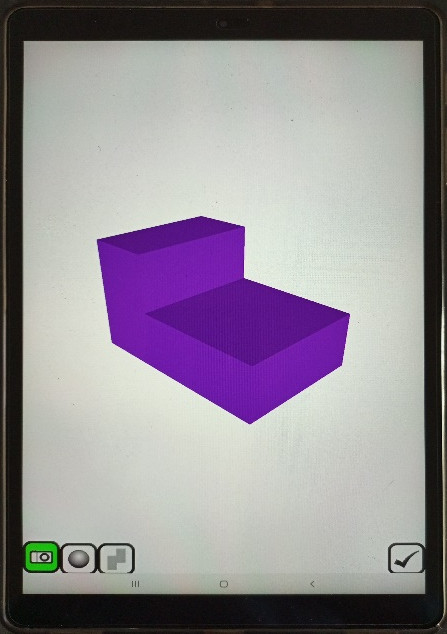
\includegraphics[width=\textwidth]{figures/figure01.jpg}
\caption{Interface do Qubism 3D Modeling.}
\label{fig-01}
\source{Elaboração própria.}
\end{minipage}
\end{figure}

\subsection{\emph{Software} de geometria dinâmica GeoGebra}\label{sub-sec-softwaredegeometriadinamica}

O software de geometria dinâmica GeoGebra, versão 5.0.721.0, é uma
ferramenta educacional livre, que permite potencializar a aprendizagem,
por meio da construção dos elementos geométricos, possibilitando a
percepção espacial da dinâmica da modelagem desses elementos. \textcite[p. 2]{alves2007} argumenta que \enquote{a utilização de softwares educativos nas
	aulas de geometria, especialmente os de geometria dinâmica, vem ao
	encontro dessas propostas, pois a utilização do computador ainda
	possibilita criar ambientes que fazem surgir novas formas de pensar e
	agir}. De acordo com o referido autor, as ferramentas do GeoGebra
permitem representar todos os conteúdos da geometria dinâmica, de modo a
impulsionar, de forma lógica, novas construções.

Particularmente para o estudo das SCs, o GeoGebra contém todos os
elementos para representar a seção produzida pelo plano secante,
permitindo esclarecer a transposição dos elementos geométricos em 3D
para 2D na folha de desenho. As ferramentas para a construção no
GeoGebra incluem ferramentas básicas de edição, pontos, transformações,
retas e polígonos (ver \Cref{fig-02}).

\begin{figure}[htpb]
\centering
\begin{minipage}{.4\textwidth}
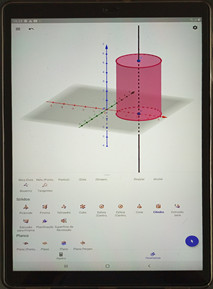
\includegraphics[width=\textwidth]{figures/figure02.jpg}
\caption{Interface do GeoGebra.}
\label{fig-02}
\source{Elaboração própria.}	
\end{minipage}
\end{figure}

\subsection{Visualização Espacial 3D}\label{sub-sec-Visualização Espacial 3D}

Visualização é o ato de observar um determinado foco, com o objetivo de
compreender todos os seus detalhes. Essa habilidade busca perceber um
objeto específico, sua composição ou ação. A Visualização Espacial é a
capacidade de observar mentalmente um determinado foco, para compreender
sua dinâmica. De acordo com \textcite[p. 2]{cohen2018},
\enquote{Consequently, these traditional psychometric spatial ability tests use
domain-general stimuli that bear little resemblance to authentic
engineering tasks} (Consequentemente, esses testes tradicionais de
habilidade espacial psicométrica usam estímulos de domínio geral, que
têm pouco em comum com tarefas de engenharia autênticas). Segundo \textcite[p. 224]{suzuki2002}, \enquote{a capacidade humana de reconhecer representações gráficas é chamada capacidade espacial ou capacidade de visualização espacial}.

Unindo os posicionamentos dos autores, VE é a habilidade de observar
espacialmente todos os detalhes do objeto, como cor, forma e posição.
Também pode ser considerada a habilidade de manipular mentalmente os
objetos no espaço para visualizar as vistas ortogonais. A capacidade
espacial nos conteúdos de Desenho Técnico e Geometria Descritiva permite
que o aluno visualize os objetos antes de resolver problemas em 2D na
folha de desenho. A habilidade espacial que se pretende que o aluno
tenha provém de um exercício mental, o que significa que, mesmo que o
aluno não tenha capacidade visioespacial, com um treinamento a partir de
exercícios progressivos e sistematizados, pode adquirir a habilidade de
VE. As disciplinas de DT e GD têm, portanto, como base, o
desenvolvimento da habilidade visual do aluno para resolver problemas de
representação e construções geométricas. Por isso, é necessária essa
habilidade para perceber mentalmente as formas e as relações dos
elementos geométricos espacialmente. Já as Projeções Ortogonais é um
tópico da disciplina de Desenho Técnico que estuda a representação de um
objeto em um plano de projeção. Uma projeção contém um conjunto de
elementos que, usando procedimentos específicos, são representados nos
planos correspondentes, permitindo diferentes vistas do objeto em
relação ao observador e proporcionando uma visão completa do mesmo
objeto através das vistas ortogonais. Por sua vez, a Seção de Cilindros
é a representação da seção produzida em um cilindro. Os elementos que
compõem a figura resultante da seção são determinados pela posição do
plano de corte.

\subsection{Mediação}\label{sub-sec-mediação}

A mediação pedagógica é um processo de interação dialógica, no qual
tanto professor quanto aluno aprendem e ensinam juntos, em construção,
pois quem ensina aprende ao ensinar e quem aprende ensina ao aprender
\cite{mori2013}. Podemos definir o processo de ensinar como uma sequência
de atividades do professor e dos alunos, visando a assimilação de
conhecimentos e o desenvolvimento de habilidades, por meio dos quais os
alunos aprimoram capacidades cognitivas, pensamento independente,
observação, análise-síntese e outras \cite[p. 54]{libaneo2013}. Por sua
vez, a aprendizagem caracteriza-se pela assimilação ativa de
conhecimentos e operações mentais, para compreendê-los e aplicá-los. É
uma forma do conhecimento humano - a relação cognitiva entre aluno e
matéria de estudo - desenvolvendo-se sob as condições específicas do
processo de ensino \cite{libaneo2013}. Na visão deste autor, a unidade
ensino-aprendizagem realiza-se na interligação de dois momentos
indissociáveis de transmissão e assimilação ativa de conhecimentos,
capacidades, em condições específicas de cada situação didática.

A mediação no ensino é o processo de aprendizagem e de interpretação dos
conteúdos planejados. Nesse processo, os intervenientes são o aluno, o
professor e a matéria. A mediação deve ser planejada com relevância para
uma prática educativa entre os intervenientes, em que o professor é o
principal agente, responsável por facilitar os conteúdos, e orientar a
construção do conhecimento no aluno, de forma colaborativa e com o
auxílio da tecnologia adequada aos conteúdos pretendidos. Vygotsky
distingue dois elementos básicos responsáveis pela mediação: o
instrumento, que tem a função de regular as ações sobre os objetos, e o
que regula as ações sobre o psiquismo das pessoas \cite[p. 50]{rego1995}.

A mediação didática deve facilitar o processo de aprendizagem e
proporcionar ao aluno uma assimilação que lhe permita construir os
conhecimentos. A realização didática tem como base a relação entre o
aluno e a matéria, com o objetivo de se apropriar dela com a mediação do
professor. O professor, nesse estágio, é um agente externo, servindo de
mediador entre o aluno e a matéria \cite{vygotskii1988}.






\section{Metodología}\label{sec-Metodología}
La presente investigación adoptó un enfoque mixto para la creación y
evaluación de ítems para ser aplicados en exámenes que evalúan el área
de Lengua Escrita, siguiendo los principios metodológicos establecidos
por autores clásicos en el campo de la educación y evaluación de
aprendizaje, como \textcite{Bloom1956} y \textcite{Messick1989}, y se incorporaron las
perspectivas sobre diseño de ítems educativos \cite{Haladyna2002}.

En este estudio, con el fin de diseñar ítems, se asignó a cuatro
diseñadores humanos y a la versión 4.0 de ChatGPT \cite{OpenAI2023} el
desarrollo de ítems para evaluar competencias en el área de Lengua
Escrita, siguiendo las teorías de evaluación educativa propuestas por
\textcite{Popham1990}. Se empleó la metodología de triangulación de datos
\cite{Denzin1978} para enriquecer la calidad y confiabilidad de los ítems
mediante la combinación de múltiples perspectivas y fuentes. Cada
diseñador humano fue responsable de la creación de 14 ítems, y ChatGPT
generó 28 ítems, totalizando 84 ítems en el área de Lengua Escrita. La
\Cref{fig01} ilustra este proceso metodológico.


\begin{figure}[htpb]
\centering
\begin{minipage}{\textwidth}
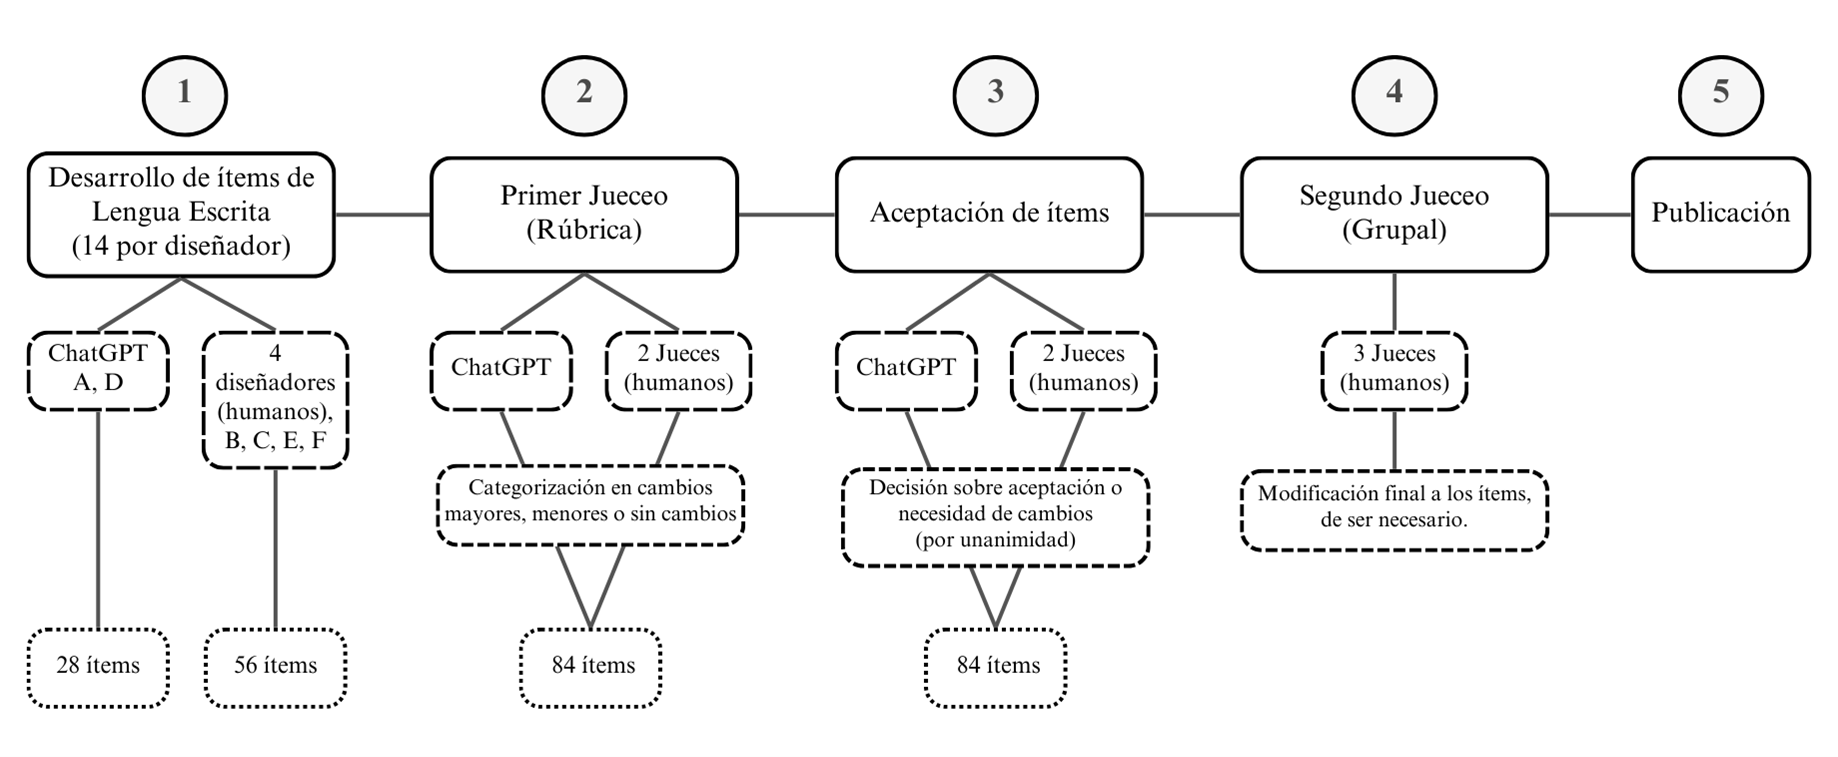
\includegraphics[width=\textwidth]{image1.png}
\caption{Proceso de evaluación y revisión de los ítems.}
\label{fig01}
\source{Elaboración propia.}
\end{minipage}
\end{figure}

Para el desarrollo de ítems se hizo uso de la IAGen ChatGPT
(\url{chat.openai.com}) en su versión de pago nombrada 4.0. Se abrieron
conversaciones por cada ítem creado, ya que todavía no estaba disponible
la posibilidad de crear un GPT con los criterios específicos para la
elaboración de ítems. En este sentido, cada ítem fue solicitado con las
características del manual de Lengua Escrita, comenzando por el uso de
la Taxonomía de \textcite{Anderson2001} para el nivel de demanda
cognitiva según la tabla de especificaciones. En cada prompt creado se
especificó:

\begin{enumerate}
	\def\labelenumi{\arabic{enumi}.}
	\item
	Identificación del contenido a evaluar
	\item
	Descripción del contenido a evaluar:
	
	\begin{enumerate}
		\def\labelenumii{\alph{enumii}.}
		\item
		Interpretación
		\item
		Ejemplos
		\item
		Delimitación del contenido
		\item
		Conocimientos y habilidades previas
		\item
		Actividades cognoscitivas
	\end{enumerate}
	\item
	Plantilla del ítem:
	
	\begin{enumerate}
		\def\labelenumii{\alph{enumii}.}
		\item
		Estructura base del ítem
		\item
		Características del texto
		\item
		Estructura y descripción de respuesta correcta y distractores.
	\end{enumerate}
	\item
	Peculiaridades de la plantilla:
	
	\begin{enumerate}
		\def\labelenumii{\alph{enumii}.}
		\item
		Base del ítem
		\item
		Vocabulario empleado
		\item
		Edición
		\item
		Peculiaridades de los distractores
	\end{enumerate}
	\item
	Bibliografía consultada y a consultar
\end{enumerate}

Por otro lado, la evaluación de los ítems fue realizada por dos jueces
humanos y por ChatGPT, siguiendo el modelo de evaluación de contenido
descrito por \textcite{Haladyna2004} y \textcite{Lynn1986}. Los jueces evaluaron cada
ítem en términos de necesidad de cambios, calidad de distractores y
aceptabilidad general del ítem. Ante esto, es importante resaltar que el
método utilizado para la evaluación de los ítems fue a doble ciego; a
ChatGPT tampoco se le indicó si quien elaboró el ítem era un ser humano
o una IAGen. Este proceso de evaluación se alinea con las
recomendaciones de \textcite{Nitko2011} sobre la importancia de una
revisión integral en la construcción de ítems de evaluación.

Los jueces evaluaron los ítems con una rúbrica (véase \Cref{tab-01}), por lo
que en esta etapa no interactuaron entre sí. Al final debían señalar si
el ítem debiese ser aceptado, aceptado con modificaciones o, bien,
podían descartarlo. Asimismo, a ChatGPT se le solicitó evaluar cada uno
de los ítems con la rúbrica disponible; es importante destacar que era
necesario tener una conversación diferente por cada ítem evaluado,
puesto que su capacidad de recordar la rúbrica era corta; es posible que
en la actualidad haya mejorado, por lo que se tiene que seguir probando
esta herramienta.



\begin{table}[!htpb]
\centering
\small
\caption{Dimensiones de la rúbrica.}
\label{tab-01}
\begin{tabular}{ll}
\toprule
Dimensiones & Elementos Clave \\
\midrule
\multirow{2}{*}{Claridad y Pertinencia del Contenido} & - Información necesaria y clara \\
    & - Tema comprensible para el público objetivo \\
\multirow{2}{*}{Neutralidad y Accesibilidad} & - Libre de sesgos\\
	& - Inclusión de imágenes/gráficas claras \\
\multirow{2}{*}{Concisión y Formato} & - Longitud adecuada del texto\\
		& - Cumplimiento de las especificaciones de formato \\
\multirow{2}{*}{Alineación Curricular} & - Congruencia con especificaciones\\
	& - Adecuación al nivel cognitivo y al público objetivo \\
\multirow{2}{*}{Claridad Disciplinar y Enfoque} & - Brevedad y claridad situacional\\
	& - Presentación directa y positiva \\
\multirow{3}{*}{Redacción y Ortografía} & - Claridad en la redacción\\
	& - Uso de vocabulario y ortografía adecuados\\
	& - Ausencia de sesgos y temas delicados \\
\multirow{3}{*}{Estructura de Respuestas} & - Uniformidad y plausibilidad de las opciones\\
	& - Ausencia de pistas indebidas\\
	& - Consistencia gramatical \\
Formato y Presentación & - Uso correcto de elementos de formato \\
\bottomrule
\end{tabular}
\source{Elaboración propia.}
\end{table}

Los resultados de las evaluaciones reflejaron una gama de decisiones,
desde la aceptación de ítems sin cambios hasta la sugerencia de
modificaciones en menor o mayor grado; o bien, el rechazo del ítem.
Estas decisiones se basaron en criterios establecidos por expertos en
evaluación educativa, como la relevancia, claridad y justicia de los
ítems \cite{Downing2003}.

Además, algunos ítems fueron seleccionados para un segundo jueceo
grupal, reflejando la metodología de revisión colaborativa sugerida por
\textcite{Stiggins2001}, lo cual permite una evaluación más profunda y detallada
en casos donde los ítems presentan desafíos particulares o requieren
ajustes más significativos. En este segundo jueceo se volvió a hacer uso
de la rúbrica, pero escuchando las observaciones de los participantes,
además se añadió a un tercer juez para tener una mejor variedad y
perspectiva sobre el jueceo.

Una vez finalizado este segundo jueceo en versión grupal, se procedió al
proceso de publicación de los ítems en su versión impresa para su
aplicación en el mes de noviembre del año 2023, como parte del proceso
de selección de ingreso a la universidad. En esta aplicación se contó
con la participación de 2,263 sustentantes, siendo 50.06~\% mujeres y
49.93~\% hombres. Los resultados de aplicación del modelo Rasch, el cual
es idóneo para medir actitudes, habilidades o personalidad
(Tristán-López, 1998), se presentan en el Anexo 1, donde todos los ítems
resultaron con índices favorables conforme a los principios de la Teoría
de Respuesta al Ítem (TRI).

Por otro lado, para el análisis del comportamiento de los jueces se
realizaron los siguientes pasos:

\begin{enumerate}[label=\Alph*)]
\item Para observar las diferencias entre el jueceo a ítems diseñados por humanos y ChatGPT
\begin{enumerate}[label=\arabic*.]
\item Preparación de datos, de forma categórica.
\item Prueba Chi-cuadrado en SPSS, siguiendo las recomendaciones de \cite{Field2013}.
\item Preparación de datos, de forma numérica para proceder a un ANOVA o
bien la prueba de Kruskal-Wallis \cite{Field2013,Howell2012}.
\item Prueba de normalidad en SPSS; el resultado fue no normal, por lo que
se procedió a la prueba de Kruskal-Wallis con las variables: Creadores
(Humano, ChatGPT), Juez A, Juez B, ChatGPT; además se aplicó la prueba
U de Mann-Whitney (Field, 2013) realizando la prueba por cada una de
las variables para revisar si había alguna variación. Todos ellos con
el \emph{software} SPSS.
\item Análisis de resultados con estadísticos básicos comparativos.
\end{enumerate}

\item Para observar la concordancia entre jueces
\begin{enumerate}[label=\arabic*.]
\item Prueba de Kappa de Cohen \cite{McHugh2012}, entre jueces: A y B, A y
ChatGPT, B y ChatGPT, a través del \emph{software} SPSS.
\item Prueba alfa de Krippendorff \cite{Hayes2007}: A, B y ChatGPT, a través del software R (Versión 2023.12.0+369), con	paquetería tidyverse e IRR.
\item Análisis de resultados con estadísticos básicos comparativos.
\end{enumerate}

\end{enumerate}
\section{Resultados}\label{sec-resultados}
\subsection{Jueceo de ítems diseñados por Humanos y ChatGPT}

Como se mencionó anteriormente, en este estudio se contemplaron dos
etapas. En este segmento se compara el resultado del jueceo según los
ítems diseñados por humanos y ChatGPT. Por un lado, se le solicitó a
ChatGPT \cite{OpenAI2023} que elaborara 24 ítems, de forma separada, pero
siguiendo los criterios marcados, y por otro, se le solicitó a cuatro
diseñadores elaborar un total de 56 ítems, 14 por cada uno de ellos. Con
el fin de evaluarlos se sometió a una revisión a doble ciego con dos
jueces humanos y un tercer juez que fue el propio ChatGPT, pero con los
parámetros de la rúbrica.

Como se describió en la metodología, se procedió a organizar la base de
datos y realizar la prueba chi-cuadrado. En la \Cref{tab-02} se pueden
observar los resultados de este primer análisis, no se observa una
diferencia significativa entre cómo evaluaron los jueces los ítems
desarrollados por humanos o por ChatGPT (Juez A, p = .758; Juez B (
.264); ChatGPT, p = 1.0). No obstante, este último, ChatGPT, muestra una
respuesta rotunda (p=1), por lo que habrá que tener cuidado sobre un
comportamiento repetitivo más que crítico.

\begin{table}[htbp]
\centering
\caption{Resultados chi-cuadrado entre ítems diseñados por humanos y
 ChatGPT según la visión de los jueces.}
\label{tab-02}
\begin{tabular}{llllp{5cm}}
\toprule
Creador & \multicolumn{1}{>{\raggedright}p{2cm}}{Chi-cuadrado de Pearson} & \multicolumn{1}{>{\raggedright}p{2cm}}{Grados de Libertad (gl)} & \multicolumn{1}{>{\raggedright}p{2cm}}{Significación Asintótica (Bilateral)} & Notas \\
\midrule
Juez\_A & 1.179 & 3 & .758 & 3 casillas (37.5~\%) tuvieron un
recuento esperado menor que 5. El recuento mínimo esperado fue .67. \\
Juez\_B & 1.247 & 1 & .264 & 2 casillas (50.0~\%) tuvieron un
recuento esperado menor que 5. El recuento mínimo esperado fue 2.33.
Solo para una tabla 2x2. \\
ChatGPT & .000 & 2 & 1.000 & 4 casillas (66.7~\%) tuvieron un
recuento esperado menor que 5. El recuento mínimo esperado fue 1.00. \\ 
\bottomrule
\end{tabular}
\source{Elaboración propia.}
\end{table}

Para complementar y teniendo los mismos resultados, se realizó la prueba
Kruskal-Wallis \cite{Field2013,Howell2012}, debido a que los resultados
de la prueba de normalidad fueron: no normal. Los resultados de la
prueba Kruskal-Wallis se observa en la \Cref{tab-03}, con los cuales se puede
confirmar que no hay diferencias significativas en las evaluaciones
(Juez\_A, Juez\_B, ChatGPT) entre los ítems creados por humanos y los
generados por ChatGPT, recordando que un valor \emph{p} menor que el
nivel de significancia elegido (0.05) indica que hay diferencias
estadísticamente significativas entre los grupos. Por ejemplo, los
resultados de Juez\_A y ChatGPT, donde los valores \emph{p} son 0.787 y
1.000 respectivamente, lo que sugiere que no hay diferencias
significativas en las evaluaciones entre los diferentes creadores de
ítems; estos resultados son similares a la realizada con chi-cuadrado
Mann Withney.

\begin{table}[htbp]
\centering
\caption{Resultados de la prueba Kruskal Wallis entre las evaluaciones de
los jueces sobre los ítems realizados entre humanos y ChatGPT.}
\label{tab-03}
\begin{tabular}{llllll}
\toprule
Variable & \multicolumn{1}{>{\raggedright}p{2cm}}{H de Kruskal-Wallis} & \multicolumn{1}{>{\raggedright}p{2cm}}{Grados de Libertad (gl)} & \multicolumn{1}{>{\raggedright}p{2cm}}{Significación Asintótica (p-valor)} & \multicolumn{1}{>{\raggedright}p{2cm}}{Prueba de la Mediana - Chi-cuadrado} & \multicolumn{1}{>{\raggedright}p{2cm}}{Prueba de la Mediana - Sig. Asintótica} \\
\midrule
Juez\_A & 0.073 & 1 & 0.787 & 0.386 & 0.534 \\
Juez\_B & 1.232 & 1 & 0.267 & 1.247 & 0.264 \\
ChatGPT & 0.000 & 1 & 1.000 & 0.000 & 1.000 \\
\bottomrule
\end{tabular}
\source{Elaboración propia.}
\end{table}

Por otro lado, se analizaron los resultados por comparación de medias,
donde se puede decir, con reservas, que los resultados del jueceo,
únicamente realizado por humanos (Juez A y B), revelan diferencias
sutiles en la aceptación de ítems entre los creados por ChatGPT y los
diseñadores humanos. En la \Cref{tab-04}, los ítems de ChatGPT mostraron una
tasa de aceptación sin cambios ligeramente superior (67.85~\%) en
comparación con los diseñadores humanos (65.17~\%). Esto sugiere que, en
términos de cumplir con los criterios establecidos inicialmente, según
los contenidos sobre Lengua Escrita, los ítems generados por ChatGPT (A
y D) se alinearon ligeramente mejor con las expectativas de los jueces.
Sin embargo, es notable que los ítems humanos (B, C, E y F) tuvieron una
tasa menor de cambios menores requeridos, pero una tasa más alta de
cambios mayores necesarios. Esto podría indicar que mientras los ítems
de ChatGPT generalmente se acercaban más a las expectativas iniciales,
los ítems humanos, cuando requerían modificaciones, necesitaban ajustes
más sustanciales.

\begin{table}[htbp]
\centering
\caption{Aceptación y comparación entre ítems realizados por humanos vs
ChatGPT (Juez A y B).}
\label{tab-04}
\begin{tabular}{lllll}
\toprule
\multicolumn{1}{>{\raggedright}p{2cm}}{Diseñadores (14 ítems por c/u)} & \multicolumn{1}{>{\raggedright}p{2cm}}{Aceptados Sin Cambios (Promedio)} & \multicolumn{1}{>{\raggedright}p{2cm}}{Aceptados Con Cambios Menores (Promedio)} & \multicolumn{1}{>{\raggedright}p{2cm}}{Aceptados Con Cambios Mayores (Promedio)} & \multicolumn{1}{>{\raggedright}p{2cm}}{Rechazados (Promedio)} \\
\midrule
%ChatGPT (A y D) & 0.6785 \textbar{} 67.8 5\% & 0.125 \textbar{} 12.5~\% & 0.1785 \textbar{} 17.85~\% & 0.0178 \textbar{} 1.7~\% \\
%Humanos (B, C, E, F) & 0.6517 \textbar{} 65.17~\% & .0625 \textbar{} 6.25~\% & .2767 \textbar{} 27.67~\% & 0.0089 \textbar{} 0.89 \% \\
ChatGPT (A y D) & 67.8 5\% & 12.5~\% & 17.85~\% & 1.7~\% \\
Humanos (B, C, E, F) & 65.17~\% & 6.25~\% & 27.67~\% & 0.89~\% \\
\bottomrule
\end{tabular}
\source{Elaboración propia.}
\end{table}

En la \Cref{tab-05}, que incluye la evaluación del Juez C (ChatGPT 4.0), se
observa un aumento en la tasa de aceptación sin cambios para ambos
grupos, siendo ligeramente más pronunciado para los ítems de ChatGPT (A
y B). Este aumento podría reflejar una alineación en la forma de evaluar
entre el ChatGPT como diseñador y como juez. Sin embargo, la tasa de
aceptación sin cambios también aumentó para los ítems humanos cuando
ChatGPT actuó como juez, lo que sugiere una evaluación consistente y
objetiva por parte de la IA. La disminución en la necesidad de cambios
menores y mayores para ambos grupos implica que el Juez C (ChatGPT) tuvo
una tendencia general a requerir menos modificaciones en los ítems.

\begin{table}[htbp]
\centering
\caption{Aceptación y comparación entre ítems realizados por humanos vs ChatGPT (Juez A, B y C).}
\label{tab-05}
\begin{tabular}{lllll}
\toprule
\multicolumn{1}{>{\raggedright}p{2cm}}{Grupo de Diseñadores} & 
\multicolumn{1}{>{\raggedright}p{2cm}}{Aceptados Sin Cambios (Promedio)} &
\multicolumn{1}{>{\raggedright}p{2cm}}{Aceptados Con Cambios Menores (Promedio)} &
\multicolumn{1}{>{\raggedright}p{2cm}}{Aceptados Con Cambios Mayores (Promedio)} &
\multicolumn{1}{>{\raggedright}p{2cm}}{Rechazados (Promedio)} \\
\midrule
%ChatGPT (A y D) & 0.7619 \textbar{} 76.19~\% & 0.0952 \textbar{} 9.52~\% & 0.1309 \textbar{} 13.9~\% & 0.0119 \textbar{} 1.19~\% \\
%Humanos (B, C, E, F) & 0.7440 \textbar{} 74.40~\% & 0.0535 \textbar{} 5.35~\% & 0.1964 \textbar{} 19.64~\% & 0.0059 \textbar{} 0.59~\% \\
ChatGPT (A y D) & 76.19~\% & 9.52~\% & 13.9~\% & 1.19~\% \\
Humanos (B, C, E, F) & 74.40~\% & 5.35~\% & 19.64~\% & 0.59~\% \\
\bottomrule
\end{tabular}
\source{Elaboración propia.}
\end{table}

No obstante, cuando se observan los resultados por diseñador, sin jueces
específicos y a partir de medias, se encuentra que no hay grandes
diferencias entre los resultados de cada uno de los diseñadores. Según
la \Cref{tab-06}, que refleja el promedio de decisiones tomadas por los tres
jueces (Juez A, Juez B y Juez C - ChatGPT 4), el 75~\% de los ítems de
todos los diseñadores fueron aceptados sin cambios, lo que indica una
alta calidad general y una alineación efectiva con los estándares de
evaluación. Este alto porcentaje de aceptación sin cambios sugiere que
la mayoría de los ítems fueron considerados adecuados y pertinentes
desde su presentación inicial. Sin embargo, hay variabilidad entre los
diseñadores, con el Diseñador B alcanzando la tasa más alta de
aceptación sin cambios (83.33~\%) y el Diseñador F la más baja (66.67
\%). Esta variación puede reflejar diferencias en los enfoques de diseño
de ítems o en la interpretación de los criterios de evaluación.

\begin{table}[!htpb]
\centering
\caption{Control de aceptación de ítems (promedio).}
\label{tab-06}
\begin{tabular}{lllll}
\toprule
\multicolumn{1}{>{\raggedright}p{2cm}}{Diseñador} & 
\multicolumn{1}{>{\raggedright}p{2cm}}{Aceptado Sin Cambios (\%)} &
\multicolumn{1}{>{\raggedright}p{2cm}}{Aceptado Con Cambios Menores (\%)} & 
\multicolumn{1}{>{\raggedright}p{2cm}}{Aceptado Con	Cambios Mayores (\%)} & 
\multicolumn{1}{>{\raggedright}p{2cm}}{Rechazado (\%)} \\
\midrule
A & 78.57~\% & 14.29~\% & 7.14~\% & 0.00~\% \\
B & 83.33~\% & 9.52~\% & 7.14~\% & 0.00~\% \\
C & 73.81~\% & 4.76~\% & 19.05~\% & 2.38~\% \\
D & 73.81~\% & 4.76~\% & 19.05~\% & 2.38~\% \\
E & 73.81~\% & 4.76~\% & 21.43~\% & 0.00~\% \\
F & 66.67~\% & 2.38~\% & 30.95~\% & 0.00~\% \\
Media & 75~\% & 6.75~\% & 17.46~\% & 0.79~\% \\
\bottomrule
\end{tabular}
\source{Elaboración propia.}
\end{table}


En cuanto a los ítems que requirieron cambios menores, la media se sitúa
en un 6.75~\%. Este porcentaje relativamente bajo indica que solo una
fracción menor de los ítems necesitaba ajustes leves para cumplir con
los criterios de evaluación. Nuevamente, existe una variación entre los
diseñadores, siendo el Diseñador B el que más a menudo requirió estos
ajustes. Los ítems que necesitaron cambios mayores presentaron una media
del 17.46~\%, lo que sugiere que, aunque en menor medida que los
aceptados sin cambios, una proporción considerable de ítems necesitó
modificaciones más sustanciales. En cuanto a la tasa de rechazo, esta
fue bastante baja, con una media del 0.79~\%, solo los Diseñadores C y D
experimentaron rechazos, aunque en una proporción mínima, lo que indica
que la gran mayoría de los ítems fueron considerados válidos y adecuados
en cierta medida.


\subsection{Consistencia y resultados entre jueces}
Sin duda, a pesar de que hubo una rúbrica como guía, como se observa en
la \Cref{tab-07}, hubo diferencias significativas entre las evaluaciones del
Juez A, B y C. El Juez A mostró un enfoque más crítico en la evaluación,
con solo un 39.29~\% de ítems aceptados sin cambios. Esta tasa más baja
sugiere un estándar riguroso o criterios más estrictos en la evaluación.
Además, un 16.67~\% de los ítems necesitó cambios menores, y una
proporción significativa, 41.67~\%, requirió cambios mayores. También se
observó un pequeño porcentaje de rechazo (2.38~\%), lo que indica que
algunos ítems no cumplían con los estándares requeridos. Por otro lado,
el Juez B adoptó un enfoque más permisivo o alineado con los diseños de
ítems, con una alta tasa de aceptación sin cambios del 92.86~\%. Esta
evaluación indulgente se refleja en la ausencia total de cambios menores
y solo un 7.14~\% de ítems que necesitaron cambios mayores. Además, no
se registraron rechazos, lo que sugiere una percepción generalmente
favorable de los ítems presentados.

\begin{table}[htbp]
\centering
\caption{Control de aceptación de ítems de los jueces.}
\label{tab-07}
\begin{tabular}{lllll}
\toprule
Juez & \multicolumn{1}{>{\raggedright}p{2cm}}{Aceptado Sin Cambios} &
\multicolumn{1}{>{\raggedright}p{2cm}}{Aceptado Con Cambios Menores} &
\multicolumn{1}{>{\raggedright}p{2cm}}{Aceptado Con Cambios Mayores} &
Rechazado \\
\midrule
Juez A & 33 \textbar{} 39.29~\% & 14 \textbar{} 16.67~\% & 35 \textbar{} 41.67~\% & 2 \textbar{} 2.38~\% \\
Juez B & 78 \textbar{} 92.86~\% & 0 & 6 \textbar{} 7.14~\% & 0 \\
\multicolumn{1}{>{\raggedright}p{2.1cm}}{Juez C (ChatGPT 4)} & 78 \textbar{} 92.86~\% & 3 \textbar{} 3.57~\% & 3 \textbar{} 3.57~\% & 0 \\
Media & 75~\% & 6.74~\% & 17.46~\% & 0.79~\% \\
\bottomrule
\end{tabular}
\source{Elaboración propia.}
\end{table}

No obstante, uno de los aspectos más relevantes fue observar la
consistencia entre los 84 ítems y los 3 jueces, el resultado fue una
concordancia baja (alfa = 0.228, véase \Cref{tab-08}), que según \textcite{Hayes2007}, el resultado varía de 0 a 1, donde valores cercanos
a 1 indican alta confiabilidad o acuerdo entre los jueces, y valores
cercanos a 0 indican lo contrario. En este sentido, como se ha analizado
anteriormente, parece existir una mayor concordancia entre el Juez B y
ChatGPT, que entre el Juez A y cualquiera de los otros dos jueces.

\begin{table}[htbp]
\centering
\caption{Resultados del alfa de Krippendorff entre los jueces.}
\label{tab-08}
\begin{tabular}{ll}
\toprule
Sujetos & 3 \\
Evaluadores & 84 \\
Alfa & 0.228 \\
\bottomrule
\end{tabular}
\source{Elaboración propia.}
\end{table}

Debido a los resultados del alfa de Krippendorf para tres jueces, se
realizó la prueba Kappa de Cohen entre los jueces A y B, y entre cada
juez y las evaluaciones de ChatGPT. Kappa de Cohen, según McHugh (2012),
es una medida de acuerdo entre dos jueces que tiene en cuenta el acuerdo
que podría ocurrir por azar. Un valor de Kappa de 1 indica un acuerdo
perfecto, mientras que un valor de 0 indica que cualquier acuerdo es
exactamente el que se esperaría por azar, y los valores negativos
indican desacuerdo. En la \Cref{tab-09} se pueden observar los resultados
entre jueces, donde:

\begin{itemize}
\item Juez A vs. Juez B: Hay un mínimo acuerdo entre estos dos jueces, que
	no es estadísticamente significativo, es decir, sus evaluaciones no
	concuerdan más allá de lo que se esperaría por azar.
\item Juez A vs. ChatGPT: Hay un mínimo, pero estadísticamente significativo
	acuerdo entre las evaluaciones del Juez A y ChatGPT. Aunque el acuerdo
	es mínimo, existe cierta concordancia más allá del azar.
\item Juez B vs. ChatGPT: Este par muestra un moderado acuerdo que es muy
	significativo estadísticamente. Indica que las evaluaciones del Juez B
	y ChatGPT concuerdan en cierta medida más allá de lo que se esperaría
	por azar. Lo que también podría significar un comportamiento
	específico a la de un humano con menos rigurosidad que, por ejemplo,
	un Juez A, más crítico.
\end{itemize}

\begin{table}[htbp]
\centering
\caption{Resultados de la prueba Kappa de Cohen entre jueces.}
\label{tab-09}
\begin{tabular}{llll}
\toprule
Comparación & Kappa & \multicolumn{1}{>{\raggedright}p{2cm}}{Significación (p-valor)} & Interpretación \\
\midrule
Juez A vs. Juez B & 0.075 & p = 0.092 & Mínimo acuerdo, no significativo \\
Juez A vs. ChatGPT & 0.089 & p = 0.017 & Mínimo acuerdo, significativo \\
Juez B vs. ChatGPT & 0.429 & p \textless{} 0.001 & Moderado acuerdo, muy significativo \\
\bottomrule
\end{tabular}
\source{Elaboración propia.}
\end{table}



\subsection{Último jueceo}
En el proceso de segundo jueceo, los resultados variaron
significativamente entre los distintos diseñadores, pero homogeneizó el
resultado final del jueceo; considerando que aquí participaron tres
jueces además del A y B y se omitió la participación de ChatGPT. En la
Tabla 6 se puede ver que para el Diseñador A, 9 de sus 14 ítems (64.29
\%) pasaron a esta etapa, con un ítem (7.14~\%) requiriendo cambios
menores y otro ítem (7.14~\%) cambios mayores, mientras que la mayoría,
7 ítems (50~\%), no necesitaron ningún cambio. De manera similar, el
Diseñador C tuvo 8 ítems (57.14~\%) en la segunda evaluación, con un
ítem (7.14~\%) necesitando tanto cambios menores como mayores, y 7 ítems
(50~\%) sin cambios. El Diseñador E también mostró un patrón parecido,
con 9 ítems (64.29~\%) en el segundo jueceo, donde 1 ítem (7.14~\%)
necesitó cambios mayores y 7 ítems (50~\%) no requirieron
modificaciones.

\begin{table}[htbp]
\centering
\caption{Resumen del control de ítems que pasaron al segundo jueceo (grupal).}
\label{tab-10}
\begin{tabular}{llllll}
\toprule
 & \multicolumn{1}{>{\raggedright}p{2cm}}{Aceptados en primer jueceo} & 
 \multicolumn{1}{>{\raggedright}p{2cm}}{Total a segundo jueceo (grupal)} &
 \multicolumn{1}{>{\raggedright}p{2cm}}{Aceptados Con Cambios Menores (Promedio)} & 
 \multicolumn{1}{>{\raggedright}p{2cm}}{Aceptados Con Cambios Mayores (Promedio)} & \multicolumn{1}{>{\raggedright}p{2cm}}{Sin cambio (Después del jueceo)} \\
\midrule
Diseñador A & 5 \textbar{} 35.71~\% & 9 \textbar{} 64.29~\% & 1	\textbar{} 7.14~\% & 1 \textbar{} 7.14~\% & 7 \textbar{} 50~\% \\
Diseñador B & 7 \textbar{} 50~\% & 7 \textbar{} 50~\% & 1 \textbar{} 7.14~\% & 0 & 7 \textbar{} 50~\% \\
Diseñador C & 6 \textbar{} 42.85~\% & 8 \textbar{} 57.14~\% & 1 \textbar{} 7.14~\% & 1 \textbar{} 7.14~\% & 7 \textbar{} 50~\% \\
Diseñador D & 4 \textbar{} 28.57~\% & 10 \textbar{} 71.43~\% & 1 \textbar{} 7.14~\% & 0 & 8 \textbar{} 57.14~\% \\
Diseñador E & 5 \textbar{} 35.71~\% & 9 \textbar{} 64.29~\% & 0 & 1 \textbar{} 7.14~\% & 7 \textbar{} 50~\% \\
Diseñador F & 3 \textbar{} 21.42~\% & 11 \textbar{} 78.57~\% & 1 \textbar{} 7.14~\% & 0 & 10 \textbar{} 71.43~\% \\
Total & 30 & 54 & 5 & 3 & 46 \\
\bottomrule
\end{tabular}
\source{Elaboración propia.}
\end{table}

Por otro lado, el Diseñador B tuvo una menor proporción de ítems que
pasaron a esta etapa, con solo 7 ítems (50~\%), y de estos, 1 ítem (7.14
\%) necesitó cambios menores y 7 ítems (50~\%) fueron aceptados sin
cambios. El Diseñador D mostró la mayor proporción de ítems en el
segundo jueceo, con 10 ítems (71.43~\%), y una alta tasa de aceptación
sin cambios, ya que 8 ítems (57.14~\%) no requirieron ajustes y solo 1
ítem (7.14~\%) necesitó cambios menores. Sobresaliendo en este proceso,
el Diseñador F presentó la mayor tasa de aceptación sin cambios, con 11
ítems (78.57~\%) pasando al segundo jueceo y 10 de ellos (71.43~\%)
aceptados tal como estaban inicialmente.

Finalmente, como se observa en la \Cref{tab-10}, la cantidad de ítems que
realmente sufrieron cambios fue un total de 8 de los 84, lo que equivale
a 9.52~\% del total. La segunda etapa de jueceo resultó muy necesaria
por la disparidad del jueceo. En este sentido, se puede concluir que el
Juez A tuvo una actitud muy crítica, lo que podría hacernos pensar en la
subjetividad del ser humano. Asimismo, en la \Cref{tab-11}, que representa el
ajuste final de los ítems después del jueceo grupal y antes de su
publicación y aplicación en un examen, se centra en los resultados
obtenidos tanto por los ítems diseñados por ChatGPT (A y D) como por los
diseñadores humanos (B, C, E, F).

\begin{table}[htbp]
\centering
\caption{Ajuste final, después de jueceo grupal, de los ítems.}
\label{tab-11}
\begin{tabular}{lllll}
\toprule
\multicolumn{1}{>{\raggedright}p{2cm}}{Grupo de Diseñadores} & 
\multicolumn{1}{>{\raggedright}p{2cm}}{Aceptados Sin Cambios (Promedio)} &
\multicolumn{1}{>{\raggedright}p{2cm}}{Aceptados Con Cambios Menores (Promedio)} &
\multicolumn{1}{>{\raggedright}p{2cm}}{Aceptados Con Cambios Mayores (Promedio)} & 
\multicolumn{1}{>{\raggedright}p{2cm}}{Rechazados (Promedio)} \\
\midrule
ChatGPT (A y D) & 85.71~\% & 7.14~\% & 3.57~\% & 3.57 \% \\
Humanos (B, C, E, F) & 89.2 8\% & 5.35~\% & 3.57~\% & 1.78 \% \\
\bottomrule
\end{tabular}
\source{Elaboración propia.}
\end{table}

Los ítems diseñados por ChatGPT mostraron una alta tasa de aceptación
sin cambios, con un 85.71~\% de los ítems considerados adecuados para su
uso sin necesidad de modificaciones adicionales. Esto indica que una
amplia mayoría de los ítems generados por ChatGPT alinearon
efectivamente con los estándares de evaluación desde su concepción
inicial. Además, un 7.14~\% de estos ítems requirieron cambios menores,
lo que sugiere que solo se necesitaron ajustes leves en una proporción
relativamente pequeña de casos. En cuanto a los cambios mayores, solo un
3.57~\% de los ítems necesitó este tipo de ajustes, y la misma
proporción (3.57~\%) fue rechazada, lo que refleja una tasa baja de
rechazo y una calidad general alta.

Por otro lado, los ítems diseñados por los diseñadores humanos
obtuvieron una tasa ligeramente superior de aceptación sin cambios,
alcanzando un 89.28~\%. Este resultado sugiere que los ítems humanos
estuvieron, en promedio, un poco más alineados con los criterios de
evaluación que los ítems de ChatGPT. Sin embargo, la diferencia no es
muy marcada, evidenciando una calidad comparable entre ambos grupos. La
tasa de ítems que requirieron cambios menores fue del 5.35~\%,
ligeramente inferior a la de ChatGPT, mientras que la proporción de
ítems que necesitaron cambios mayores fue idéntica a la de ChatGPT, 3.57
\%. La tasa de rechazo para los ítems humanos fue del 1.78~\%,
ligeramente inferior a la de ChatGPT, lo que indica un margen muy
estrecho en términos de calidad y aceptación general.

\section{Conclusão}\label{sec-conclusão}

As tecnologias 3D são primordiais para a visualização 3D dos sólidos
geométricos, promovem a VE no estudo de vários temas de Desenho Técnico,
oferecendo simulações de experiências virtuais em tempo curto, assim
sendo, permitindo repetições das experiências e com baixo custo. Essas
experiências devem-se ao rápido desenvolvimento das tecnologias nos
últimos anos, em que se assistiu a muitas invenções de dispositivos
tecnológicos e de informação e criação de programas espaciais de
modelação 3D.

O AT Q3DM é uma ferramenta com potencial para o estudo das POs, porque é
adequado aos conceitos de representação das VOs resultantes da sua
projeção. Dessa forma, estimula a aprendizagem dos alunos, por meio da
sua apresentação interativa com alta resolução de nitidez dos elementos
geométricos.

O AT de geometria dinâmica GeoGebra é um meio didático que gerou grande
interesse e motivação nos alunos nas atividades de resolução de SCs. Por
conseguinte, promoveu a VE da seção produzida em qualquer posição do
plano secante no cilindro.

Respondendo à questão de investigação, os alunos melhoraram a VE no
estudo das POs e Scs, por meio de simulações computacionais de
exercícios práticos em 3D em ATs. Assim sendo, os alunos simularam os
exercícios de forma interativa e dinâmica, o que facilitou o transporte
para a folha de desenho. Portanto, foi observada uma redução de
dificuldades e um desenvolvimento de habilidades de VE. Os pressupostos
da pesquisa interpretativa possibilitaram adentrar no mundo social dos
alunos, para compreender, em diversas situações, qual o significado de
suas ações. A tecnologia na sala de aula pode garantir bons resultados,
porque permite uma representação de todos os elementos de DT e GD, mas
não substitui o professor, porque o professor é o agente que desenvolve
situações no ensino e integra a tecnologia relacionada com o
conhecimento pretendido na aprendizagem.




\section*{Agradecimentos}\label{sec-agradecimento}

O primeiro autor agradece à Fundação Calouste Gulbenkian, no âmbito do
programa de apoio à formação dos PALOP e de Timor-Leste. Além disso, o
último autor agradece aos Fundos Portugueses, através da FCT Fundação
para a Ciência e a Tecnologia, no âmbito dos Projectos UIDB/00013/2020,
UIDP/00013/202.


\printbibliography\label{sec-bib}
%conceptualization,datacuration,formalanalysis,funding,investigation,methodology,projadm,resources,software,supervision,validation,visualization,writing,review
\begin{contributors}[sec-contributors]
\authorcontribution{Cacilda Helena Chivai}[conceptualization,funding,investigation,software,writing,review]
\authorcontribution{Armando Assunção Soares}[formalanalysis,resources]
\authorcontribution{Paula Catarino}[methodology,projadm]
\end{contributors}
\end{document}
